\documentclass[12pt]{report}
\renewcommand{\chaptername}{Kapitel}
\usepackage{a4}
\usepackage{color}
\usepackage[T1]{fontenc}
\usepackage[danish]{babel}
\usepackage[hidelinks]{hyperref}
\usepackage{lingmacros}
\usepackage{tree-dvips}
\usepackage{url}
\usepackage{graphicx}
\usepackage{float}

\definecolor{Red}{RGB}{255,0,0}
\begin{document}

\begin{titlepage}

\newcommand{\HRule}{\rule{\linewidth}{0.5mm}} 

\center

\textsc{\LARGE Aalborg Universitet}\\[1.0cm]
\textsc{\LARGE B228}\\[1.0cm]
\textsc{\Large P1-Rapport}\\[0.0cm]
\textsc{\large Statusseminar}\\[0.5cm] 

\HRule \\[0.4cm]
\center { \huge \bfseries Komprimering af korte beskeder}\\[0.4cm]
\HRule
 
\begin{flushleft} \large
\emph{Forfattere:}\\
Jannek Alexander Westerhof \textsc{Bossen} \\
Kevin \textsc{Br�mer} \\
Frederik Meyer \textsc{B�nneland} \\
Rikke \textsc{Holmberg} \\
�lavur Debes \textsc{Joensen} \\
Anders Trier \textsc{Olesen} \\
Katrine Sofie \textsc{Tjell} \\
\end{flushleft}
 

\begin{flushleft} \large
\emph{Vejledere:} \\
Michael Sk�tt \textsc{Madsen} \\ % Supervisor's Name
Amanda \textsc{Hill} \\% Supervisor's Name
\end{flushleft}


\vfill
{\large \today}\\[1cm]





\end{titlepage}

\chapter*{L�sevejledning}
I de f�lgende arbejdsblad er de vigtigste dele af vores analyse ang�ende komprimering af korte beskeder. Den skulle gerne hj�lpe til at give et overblik over hvad vi har t�nkt os at lave med vore projekt. Det f�lgende er en lille liste opstillet i punktform over de aspekter af vores projekt vi is�r gerne vil have feedback p�.

\begin{itemize}
Bliver metoderne brugt, p� en s�dan m�de at det er relevant for projektet? 
Hvordan kan vi g�re vores projekts kontekst bedre?
Er det muligt at benytte andre eller bedre analyse metoder?
Kan delproblemerne l�ses med l�sningsformer der fungerer bedre i disse tilf�lde?
\end{itemize}
\chapter*{Arbejdsblade}
\section*{Indledning}

I 1992 blev den f�rste SMS afsendt \cite{museum}. Dengang kunne denne type tekstmeddelse maksimalt rumme 160 tegn, hvilket er n�jagtig lige s� mange tegn, som en SMS kan indeholde i dag. Det var den tyske engin�r Friedhelm Hildebrand, der i 1985 s� potentialet i muligheden for at sende korte tekst beskeder fra mobiltelefon til mobiltelefon. Han unders�gte hvor mange tegn der normalt blev brugt n�r man skrev et postkort, ligesom at han selv skrev forskellige beskeder, som han forstillede sig, at folk ville skrive til andre via deres mobiltelefon. Hverken antallet af tegn p� postkortene, eller antallet af tegn i de korte beskeder Hillebrand selv skrev oversteg 160 tegn. Derfor blev gr�nsen for hvor mange tegn en SMS kan indeholde sat ved 160.
Gennem tiden har meget teknologi �ndret sig, s� m�ske burde man i dag have muligheden for at sende flere end 160 tegn i en SMS. \cite{hillebrand}

\subsubsection {Datakomprimering}

Datakomprimering handler om at g�re en datam�ngde mindre. Der kan b�de v�re tale om filer, billeder, film osv.. Man �nsker ofte at data skal fylde s� lidt som muligt, derfor er komprimering et meget centralt emne indenfor datalogi. N�r man eksempelvis taler om hukommelseslager, computernetv�rk, herunder is�r internettet, er det meget relevant at data fylder s� lidt som muligt.
 
Man kan komprimere enkelte filer s�vel som hele samlinger af filer. Mange siger ofte at filer pakkes, n�r man komprimerer. Der findes allerede flere komprimeringsprogrammer; zip, jpeg, WinZip, SMS ZIP, SMS ZIPPER, for bare at n�vne nogle f�.

Der findes selvf�lgelige mange m�der at komprimere p� og lige s� mange forskellige komprimeringsalgoritmer. Disse algoritmer kan deles op i to kategorier, tabsfri og ikke-tabsfri.  
Det man ofte udnytter n�r man komprimere tabsfrit, er at de fleste m�ngder af data indeholder den samme information flere gange. Eksempelvis indeholder en tekstfil de samme ord gentagne gange. Derfor kan man i stedet for den gentagne information skrive informationer om hvor mange gange den bestemte information er blevet gentaget. P� den m�de kan dataene genskabes uden tab. Denne kategori benyttes is�r til tekstfiler, hvor det er s�rlig vigtigt at filen kan genskabes 100 procent. Ikke-tabsfri kompression kan eksempelvis benyttes til billedkomprimering, hvor det kan g� an at ikke hver pixel genskabes 100 procent.
\subsubsection*{Initierende Problem}


Der er forskellige tjenester der giver mulighed for at skrive korte tekstbeskeder. Fælles for dem alle er, at det kun er tilladt at skrive et begrænset antal tegn pr. besked, hvis denne grænse overskrides deles beskeden i to. Problemet er, at hvis der eksempelvis er tale om en SMS besked, kommer man til at betale dobbelt SMS takst, hvis beskeden bliver delt i to.


\section*{Problemafgr�nsning}
Dette afsnit kommer omkring nogen af de valg, der blev lavet for at indskrænke projektets problemfelt. For det første er der forskellige tjenester og teknologier, som giver muglihed for at sende en kort besked, men med et begrænset antal tegn pr. besked. Eksempelvis er der SMS-beskeder med en begrænsning på 160 tegn når man bruger tegn fra tegnsættet GSM 7-bit\cite{Pro_1} og der er også internettjenester som for eksempel Twitter, som har en tegnbegrænsning på 140 tegn\cite{pro_af1}. Twitters formål har fra starten af, været at give mulighed for at sende korte og smertefrie bidder af information over internettet, og ikke lange blogs og artikler. Denne holdning er folkene bag Twitter meget konsekvente med\cite{pro_af2}. Derudover så er det også gratis at gøre brug af Twitter og derfor er det ikke ligeså væsentligt som SMS, som koster penge. Derfor har vi valgt ikke at arbejde med Twitter. Istedet vil projektet blive begrænset til at handle om SMS-beskeder.

Nu hvor valget om SMS eller Twitter er på plads, så kommer spørgsmålet om hvorvidt der skal arbejdes med smartphones eller almindelige mobiltelefoner. Smartphones har den fordel, at de kan implementere applikation uden alt for meget besvær, hvorimod på almindelige telefoner er det mere besværligt at installere programmer. Statistikkerne viser at flere og flere begynder at få smartphones\cite{pro_af3}. I det sidste kvartal af 2011 blev der solgt over 37 millioner iPhones, Apple's smartphone, i hele verdenen, som er højere end antallet af børn født i den samme periode\cite{pro_af4}. Derudover så bliver der også vist, at brugen af hjemme computere er dallende i det, at adgang til internettet også er tilgængeligt gennem smartphones, som derved gør det muligt for en person at være på internettet hvor man ellers ikke ville have tilgang til en almindelig computer\cite{pro_af3}. Dette kan betyde, at flere personer bruger SMS, fordi de bruger deres mobile enheder mere. Dog kan det også betyde at flere mennesker bruger e-mail i stedet for SMS fordi de alligevel har adgang til internettet. Ud fra dette vil projektet yderligere blive begrænset, til ikke at prøve at implementere programmet på almindelige mobiltelefoner. Derudover så er det også vanskeligt, at implementere en applikation skrevet i C, som er et krav for dette projekt, på en smartphone. Derfor vil løsningen være en prototype, som kan fungere på en computer. 

Når løsningen skal laves, er der brug for en komprimeringsalgoritme. Tidligere er et par komprimeringsalgoritmer blevet gennemgået, for eksempel Huffman eller PPM, som kan bruges til at udvikle løsningen. PPM løsninger har det med at være de bedste til komprimering af tekst. Ligeledes er komprimeringskraften ved Huffman for sig selv også meget kraftig, men er ikke altid optimal. Det er muligt at bygge ovenpå en Huffman komprimeringsalgoritme med PPM. PPM har dog et behov for en del mere RAM i forhold til Huffman, for at kunne komprimere, og er også en langt mere kompliceret løsning at udvikle. Ud fra projektets rammer samt den teoretiske platform som løsningen skulle kunne køre på, en mobiltelefon, så er Huffman løsningen den bedste mulighed. Derfor vil løsningen blive indskrænket til at bruge Huffman som komprimeringsalgoritme.\cite{pro_af5}

Løsningen skal kunne køre uden at forstyrre brugeren af programmet alt for meget. Her gælder blandt andet den tid det tager for programmet at komprimere beskeden, samt hvor meget plads og regnekraft det tager. Det er blandt andet derfor, at det blev besluttet løsningen skulle udvikles ud fra Huffman alene, og ikke lave løsningen med PPM. Ligeledes så skal det heller ikke være nødvendigt for brugeren selv at gøre noget for at komprimere beskeden. Komprimering skal ske automatisk i SMS-processen, uden at brugeren behøver at sætte det igang. Hvis det er nødvendigt med yderlig bruger interaktion, så skal det foregå så brugervenligt som muligt.

Det sidste punkt er hvilke tegnsæt som løsningen skal være i stand til at komprimere og dekomprimere. Skal tegn fra det kyrilliske alfabet eller specialtegn som Æ, Ø, Å og ß være i stand til at blive komprimeret, for eksempel. Det er blevet bestemt, at løsningen skal have implementeret GSM 7-bit tegnsættet, som er standard tegnsættet til SMS-beskeder på mobiltelefoner og smartphone.

\section*{L�sningsforslag}
L�sningsforslag
Vi har formuleret et initierende problem, som handler om hvordan man kan spare penge p� at sende sms'er.

Prisen p� sms'er

En oplagt l�sning er selvf�lgelig at f� prisen p� afsendelse af sms'er sat ned. Dette kan enten ske ved at de forskellige teleselskaber satte priserne ned, m�ske med det form�l at vinde en st�rre del af markedet. En anden m�de det kan ske p�, er ved lovgivning.

Begr�nsningen p� tegn

En anden l�sning p� problemet er, at s�rge for at hver forbruger skal afsende s� f� sms-beskeder som muligt. Som det fungerer i dag, sendes der �n sms-besked for hver p�begyndt 160 tegn. Det vil sige, at hvis en forbruger skriver en sms p� 200 tegn, ville denne deles op og sendes som to. Hvis disse beskeder eksempelvis skal sendes til udlandet, bliver det pludseligt til mange penge.
En m�de man kan forhindre dette p�, er at s�rge for at begr�nsningen p� tegn bliver �ndret s�ledes at man kan sende flere end 160 tegn pr. sms.
En anden mulighed er at komprimere sms-beskederne, for p� den m�de, at f� en sms-besked p� 200 tegn, til at fylde 160 tegn eller f�rre. Herved undg�r man at betale for afsendelse af to beskeder, n�r man egentlig bare vil sende �n.
 
Diskussion
Den f�rste l�sning, som handlede om at f� sat prisen p� sms'er ned kan v�re sv�rt at realisere. Man m� n�sten g� ud fra at selskaberne allerede har en s� konkurrencedygtig pris som muligt, s� det er usandsynligt at de frivilligt skulle s�tte sms taksten ned. Hvis det blev gennemf�rt ved lovgivning, ville selskaberne sikkert bare finde en anden vej til at f� pengene hjem, eksempelvis ved h�vet eller indf�relse af nye afgifter.
Den n�ste l�sning handlede om at f�  �ndret begr�nsningen af antal tegn pr. sms besked. Den l�sning ville kr�ve en �ndring i sms teknologien og vil derfor ikke v�re noget vi kan besk�ftige os med i dette projekt. Den sidste l�sning handler om at komprimere sms-beskeder. Dette vil kr�ve at den mobiltelefon som skal afsende sms-beskeden har et program der netop kan komprimere, men samtidigt kr�ve at den telefon som skal modtage beskeden har et tilsvarende program, som kan dekomprimere beskeden.

\section*{Kontekstualisering}
I forbindelse med projektet er der blevet t�nkt over en r�kke metoder, som g�r os i stand til at finde ind til vores problems kerne, og underst�tte problemet i sin helhed.
Ud fra projektforslaget er det blevet fastsat at vores endelige l�sning til problemet skal v�re en prototype af et program. Denne prototype skal v�re skrevet i C, men da problemstillingen omhandler SMS-beskeder, er det  SMS-mediets krav, som vi skal designe vores l�sning efter.


Ud fra vores problem findes der en r�kke interessenter, som p�virkes af denne problemstilling.
P� den f�lgende brainstorm, ses hvordan disse interessenter fordeler sig, ud fra det initierende problem, og hvordan de forbindes til hinanden.

\begin{figure}[H]
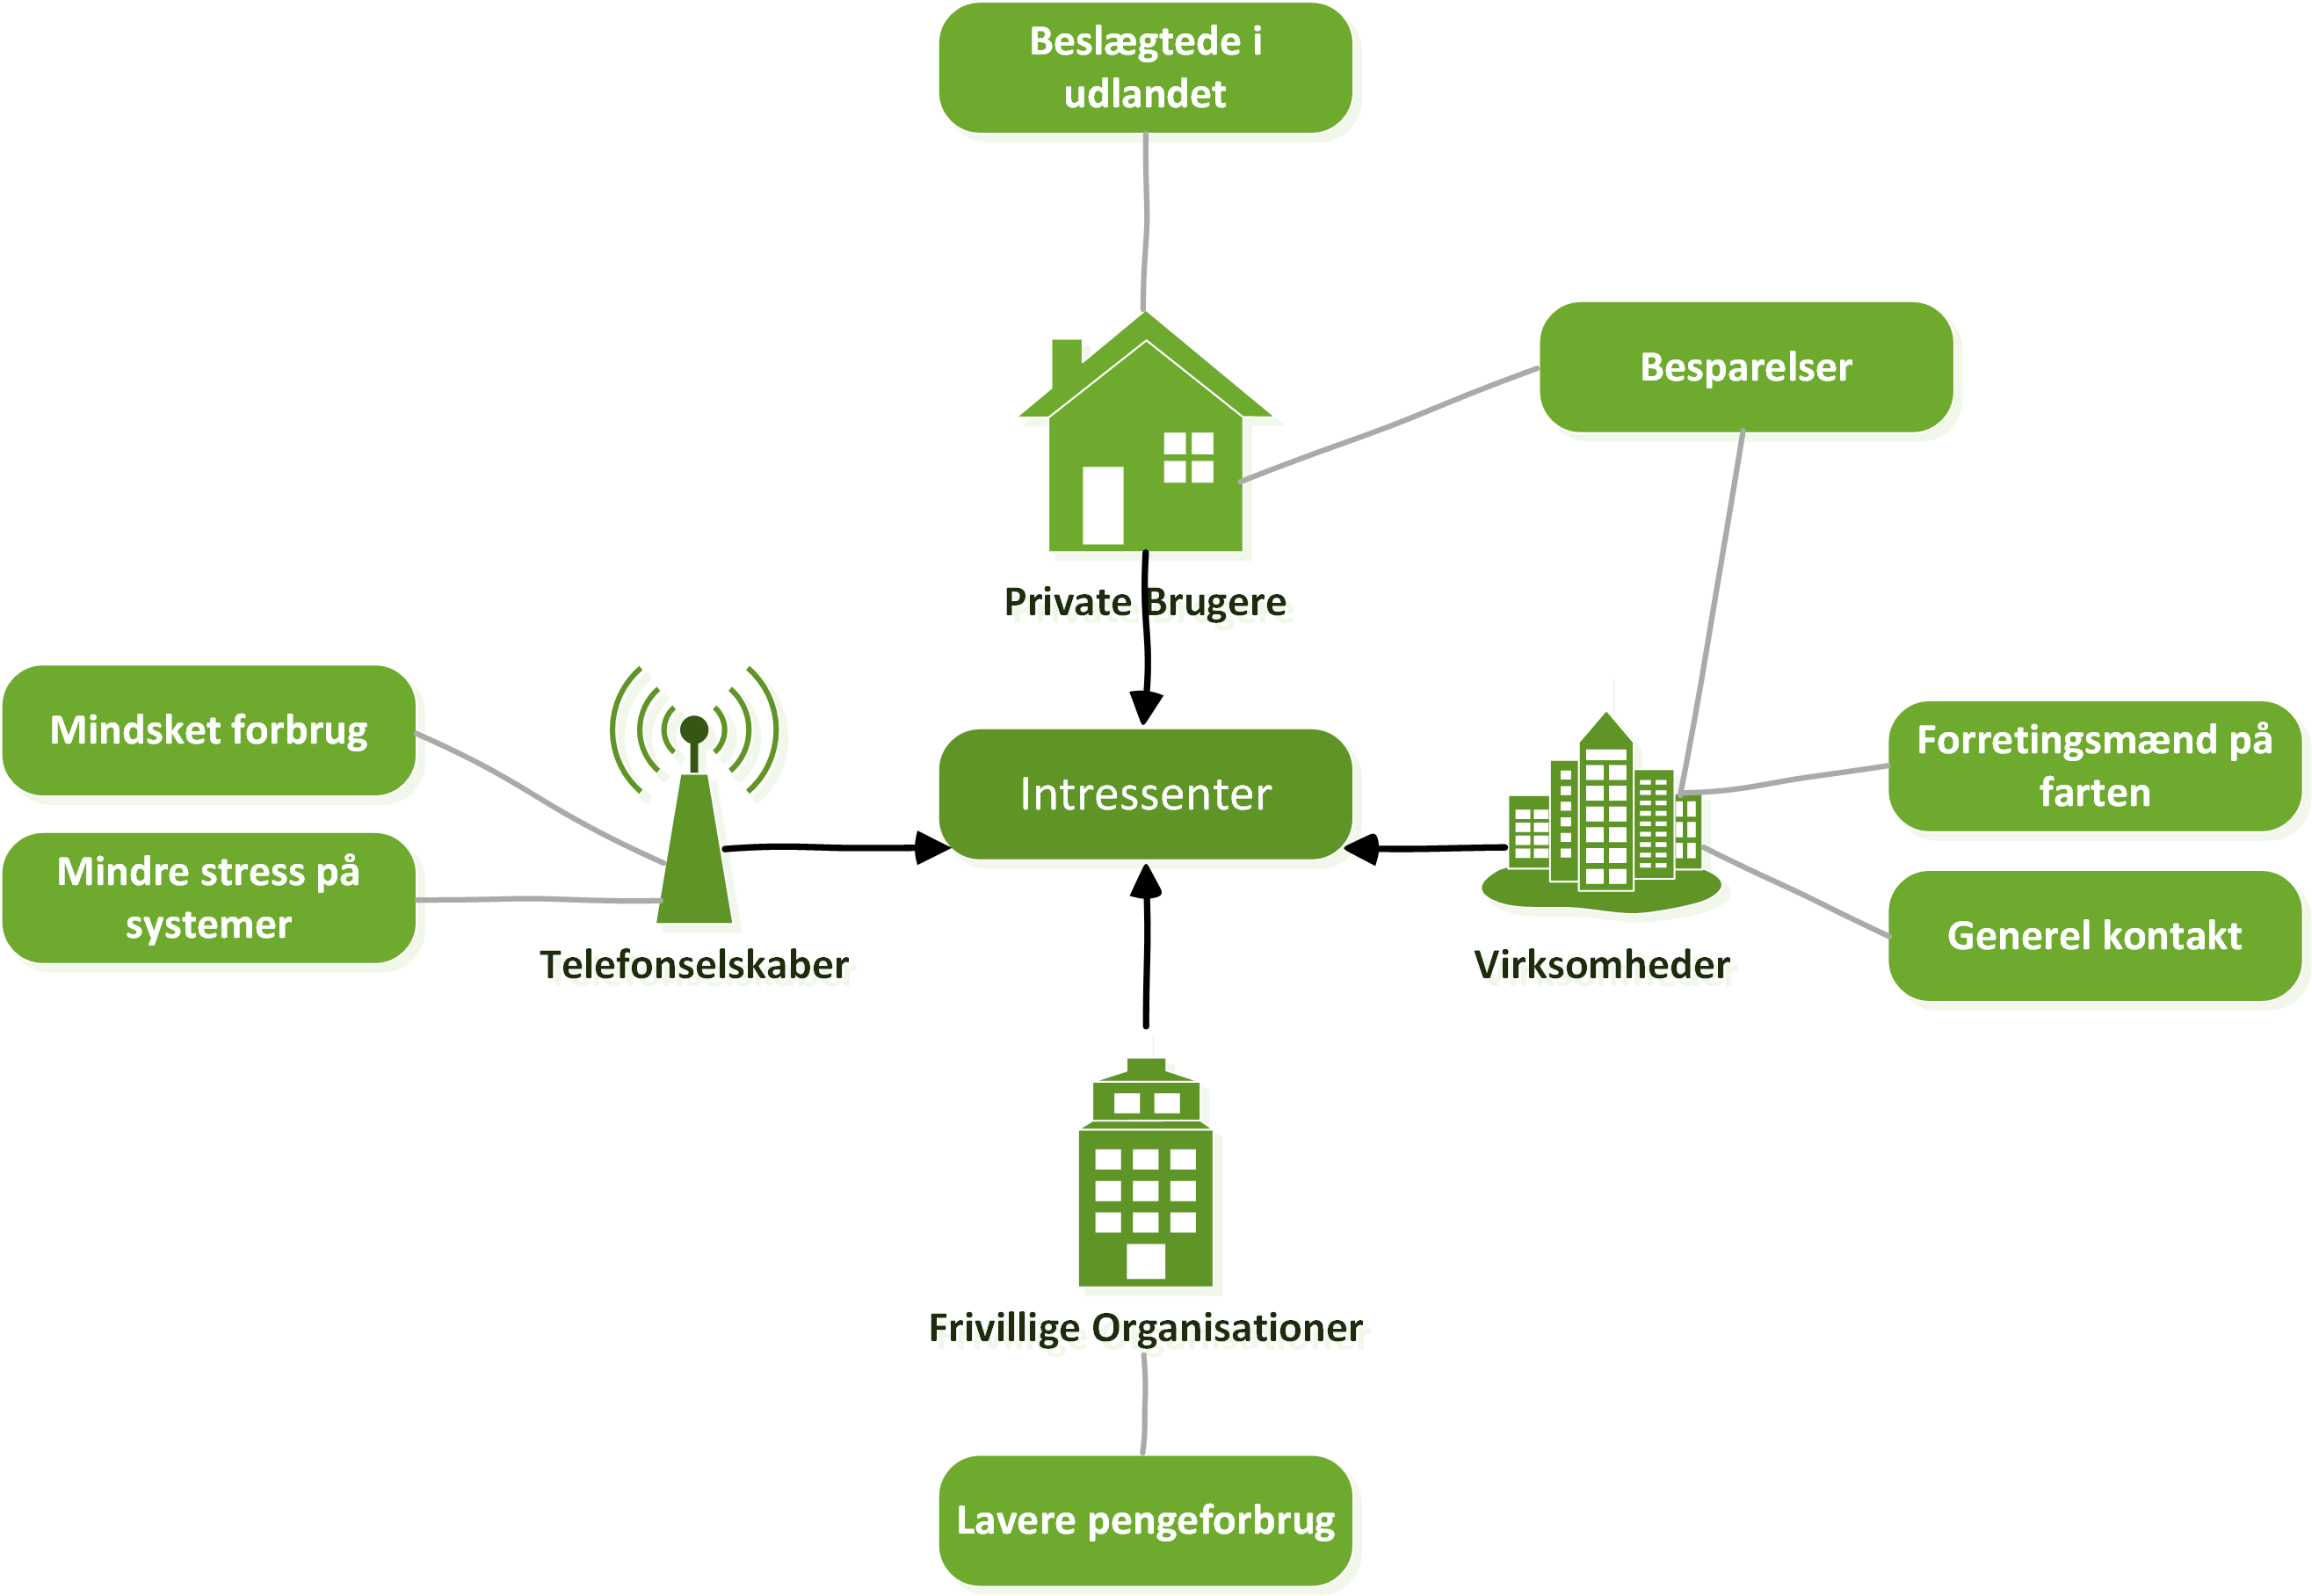
\includegraphics[width=\linewidth]{Billeder/Brainstormting.png}
\caption{Her ses hvordan interessenterne fordeler sig.}
\end{figure}

Denne brainstorm identificerer vores prim�re interessanter, som vil v�re vores hovedm�lgruppe.
Man kan dele interessenterne ind i nogle grupper, henholdsvis: Private personer, Internationale firmaer, Frivillige organisationer og Teleselskaber.
Hver af disse grupper har sin egen grund til at v�re interesseret i vores problemstilling, og derfor kan det ogs� betyde, at der skal forskellige l�sninger til at kunne l�se problemstillingen, for hver forskellig interessant.


Ud fra vores problemstilling findes der en r�kke data som kan v�re anvendelig i forhold til unders�gelsen af de f�rn�vnte interessenter.


Viden om brugen af SMS?er hos de forskellige interessent grupper.
Det er vigtigt at finde ud af hvordan de forskellige interessenter bruger SMS?er som et medie. Med dette menes b�de hvor tit det bruges, men ogs� i hvilken forbindelse og med hvem kommunikationen foreg�r.


Til indsamling af data omkring disse interessanter er det n�dvendigt at komme i direkte kontakt med den m�lgruppe vi har med at g�re. Dette betyder at vi bliver n�dt til at benytte nogle metoder, som g�r det muligt at indsamle eller observere m�lgruppens forbrug af SMS?er.
Til dette vil en sp�rgeskema unders�gelse v�re velegnet, da brugen af SMS?er er data velegnet til kvantitative unders�gelser, da det er et sp�rgsm�l om hvor mange SMS?er der sendes.

\subsubsection{Eksisterende L�sninger}
Der findes flere forskellige former for programmer der allerede helt eller delvist l�ser sms- begr�nsnings problemet. Vi vil i det f�lgende afsnit tage udgangspunkt i to eksisterende programmer.

Det f�rste program hedder SMS ZIP og virker kun til smartphones med Windows som operativsystem. Dette program er af typen ikke tabsfri, da det g�r ind og fjerner alle un�dige mellemrum i teksten, og erstatter f�rste bogstav i f�lgende ord med et stort bogstav, s�ledes at teksten stadig kan l�ses. Ydermere er det programmeret til at kunne identificere bestemte ord og s� erstatte disse med forkortelser. Programmet er indrettet s�ledes at brugeren selv skal v�lge om hver enkelt besked skal komprimeres. Et eksempel p� hvordan programmet vil komprimere en besked:\cite{download-sms} 
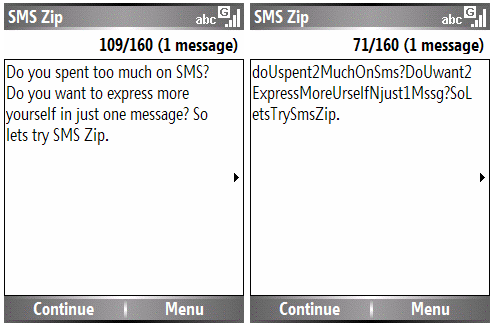
\includegraphics []{Billeder/SMSZIP.png}

Denne konkrete besked bliver alts� kortet ned fra 109- til 71 tegn. En af fordelene ved dette program er at modtageren ikke beh�ver et tilsvarende dekomprimeringsprogram for at kunne l�se beskeden. En anden fordel er at beskeder der ikke overg�r en begr�nsningen, ikke n�dvendigvis bliver komprimeret. Denne l�sning har dog en del flere ulemper end fordele. Den �benlyse ulempe er at beskederne bliver en hel del sv�rere at l�se, og kan v�re en mulig irritation for mange, n�r de l�ser beskeden. En anden klar ulempe er at der bliver brugt en del slang for at g�re ordene kortere, slang s�som tallet ?2? i stedet for ordet ?to?. Dette kan bevirke at budskabet er sv�rere at tage seri�st. Yderligere er det et problem at programmet kun virker til windowsphones og at forkortelserne kun er beregnet til engelsktalende beskeder. Det er derfor, p� baggrund af ovenst�ende, vores vurdering at programmet er en ufuldst�ndig l�sning, og er derfor ikke tilstr�kkelig.\cite{download-sms}

En anden eksisterende l�sning hedder SMS ZIPPER. Det er p� mange punkter et totalt modstridende program i forhold til SMS ZIP. F�rst og fremmest er det forskelligt da dette er et tabsfrit komprimerings program. Programmet virker p� langt de fleste smartphones og er, i mods�tning til SMS ZIP, en l�sning der komprimerer beskeden hos afsenderen og derefter dekomprimerer beskeden igen hos modtageren. Dette kr�ver dog at b�de afsender og modtager har programmet installeret. Programmet starter p� modtagerens telefon liges� snart en komprimeret besked modtages, s� beskeden kan l�ses med det samme uden besv�r for l�seren. Producenten lover helt op til 480 tegn pr. besked, alts� 3 gange s� mange tegn som en almindelig sms. Derudover fungerer programmet til flere sprog, heriblandt dansk, engelsk og tysk.\cite{smszipper} 

Dette program bruger en fleksibel algoritme til at komprimere beskederne. De har designet algoritmen direkte med henblik p� s�kaldte korte beskeder, alts� beskeder omkring de 160 tegn. Endvidere bruger programmet ogs� andre kodnings modeller, som kan v�re beregnet specifikt p� bestemte sprog eller typer af beskeder.

Vi har i ovenst�ende afsnit valgt at tage to vidt forskellige programmer under luppen, for at tegne en kontrast mellem en meget simpel og en mere avanceret l�sning. Vi ser at de hver is�r har deres fordele og ulemper, og disse vil vi tage til overvejelse i vores program.

\section*{Problemformulering}
Ud fra vores problemanalyse har vi fundet ud af, at der klart er penge at spare, hvis man fra udlandet kan sende én besked i stedet for to. Vi har ligeledes set på eksisterende løsninger som SMS ZIP, for at undgå at lave de fejl, vi mener der er ved de programmer. Derudfra skal vores løsning være mere implementeret, således at brugeren aldrig kommer til at beskæftige sig med den komprimerede besked, så komprimering og dekomprimering sker automatisk. Vi er på baggrund af dette kommet frem til følgende problemformulering:

\begin{itemize}
\item[] \emph{Hvordan kan man spare forbrugeren for dobbelt SMS-takst, ved brug af et komprimeringsprogram? Hvordan kan man undgå at programmet bliver en belastning for brugeren?}
\end{itemize}

Der vil arbejdes frem mod en prototype, der kan komprimere en kort besked, for siden at dekomprimere den på en anden enhed. 

\clearpage

\documentclass[12pt]{report}
\renewcommand{\chaptername}{Kapitel}
\usepackage{a4}
\usepackage{color}
\usepackage[T1]{fontenc}
\usepackage[danish]{babel}
\usepackage[hidelinks]{hyperref}
\usepackage{lingmacros}
\usepackage{tree-dvips}
\usepackage{url}
\usepackage{graphicx}
\usepackage{float}

\definecolor{Red}{RGB}{255,0,0}

\begin{document}

\chapter*{Gruppekontrakt}
\section*{Ambitionsniveau}
Der er fastsat h�jt ambitionsniveau i gruppen.
\section*{M�dedisciplin}
Der er m�depligt ved alle m�der, b�de vejlederm�der og gruppem�der.
Man har pligt til at melde afbud, hvis man ikke kan komme. Dette g�lder ogs� hvis man ikke kommer til en forel�sning.
\section*{Fredagshygge}
Der er aftalt at der hver fredag medbringes kage, for at �ge motivationen. Gruppemedlemmer har skiftevis ansvar for at medbringe kage, hvilket foreg�r i f�lgende r�kkef�lge:
\begin{enumerate}
	\itemsep1pt \parskip0pt \parsep0pt
	\item Anders
	\item Rikke
	\item �lavur
	\item Frederik
	\item Jannek
	\item Katrine
	\item Kevin
\end{enumerate}
\section*{Tidsplaner og Deadlines}
Projektets ultimative deadline ligger onsdag d. 19. december. Der vil dog fremg� del-deadlines i tidsplanen. Dette bevirker endvidere at alle i gruppen, p� ethvert tidspunkt er afklaret med hvad der skal laves.
\section*{Problemer og Konflikter}
Det er op til det enkelte gruppemedlem at f� den p�g�ldendes arbejde f�rdigt til tiden. Det er derfor op til det enkelte gruppemedlem at sige til hvis han/hun ikke er helt afklaret om arbejdsopgaven. Der er dog mulighed at samarbejde om opgaver hvis det er n�dv�ndigt. Ydermere er det op til det enkelte gruppemedlem at give status p� en arbejdsopgave ved gruppem�der.
\section*{M�destruktur}
Der vil ved m�der v�re en dagsorden, der er fastlagt p� forh�nd. Det er dog muligt at lave tilf�jelser til dagsordenen under m�det om n�dv�ndigt. Under vejlederm�der vil der blive udvalgt en referant der tager noter under m�det. Efter m�der vil der blive reflekteret over m�det og det videre arbejde vil blive dr�ftet samt uddeling af arbejdsopgaver.
\end{document}

\begin{thebibliography}{99} %Max
 \bibitem{A_Method_for} D.A. Huffman, {\it Proceedings of the I.R.E.}, September 1952.




%Eksempel:
%\bibitem{DandJ} Dow, W. \& Jones, E.A., {\it Wall Street Journal}, March 29, 1929.

%Eksempel2:
%\bibitem{Simpson} H. Simpson, \emph{Proof of the Riemann
%Hypothesis},  preprint (2003), available at 
%\url{http://www.math.drofnats.edu/riemann.ps}.
\end{thebibliography}
\end{document}
